\chapter{Ist-Situation der Hochschule Emden/Leer hinsichtlich wichtiger Dimensionen - ME, TK}
\textit{Autoren: Marc Enders (ME), Tina Koppermann (TK)}

Im Folgenden wird auf die Ist-Situation an der Hochschule Emden/Leer eingegangen. Durch ein 
Experteninterview mit dem Leiter des Hochschulrechenzentrums sowie weiteren intensiven Recherchen soll 
mit Hilfe der gesammelten Informationen reflektiert werden, ob an der Hochschule bereits ein 
Informationsmanagement betrieben wird. Anschließend erfolgt eine Bewertung und Gewichtung der 
bisherigen Ist-Situation.

Im Folgenden wird auf die Ist-Situation an der Hochschule Emden/Leer eingegangen. Durch ein 
Experteninterview mit dem Leiter des Hochschulrechenzentrums sowie weiteren intensiven Recherchen soll 
mit Hilfe der gesammelten Informationen reflektiert werden, ob an der Hochschule bereits ein 
Informationsmanagement betrieben wird. Anschließend erfolgt eine Bewertung und Gewichtung der 
bisherigen Ist-Situation.

\section{Ziel (TK)}
Mit Hilfe einer Analyse der Ist-Situation an der Hochschule Emden/Leer wird festgestellt, in wieweit bereits 
ein Informationsmanagement besteht. Wenn dies nicht der Fall ist, wird recherchiert, welche Informationen 
zentral gesammelt werden und welche Bereiche in das Projekt \textbf{„Potentielle Neuordnung des 
	Informationsmanagements einer kleineren Fachhochschule auf der Grundlage bestehender Lösungen an 
	deutschen Hochschulen“} mit einbezogen werden müssen.

Wesentliche Fragestellungen, die in diesem Kapitel gelöst werden sollen, sind auf der einen Seite, 
herauszufinden, welche vorhandenen IT-Systeme bereits zentral Verwendung finden und auf der anderen 
Seite, wie Informationen aktuell repräsentiert werden. Des weiteren soll in dieser Analyse Aufschluss darüber 
gegeben werden, ob ein Informationsmanagement an der Hochschule betrieben wird und wie Informationen 
bereits zentral zur Verfügung gestellt werden.

Die Hochschule Emden/Leer ist eine kleine Hochschule mit aktuell 4626 eingeschriebenen Studierenden. Den 
größten Anteil machen die 4303 Studenten vor Ort 
aus.\footcite{hsel_zeitreihe_2014} Die Hochschule beschäftigt 396 
Mitarbeiter.\footcite{hsel_zdf_2015}
\section{Methodisches Vorgehen (TK)}
Ein Hauptbestandteil dieses Kapitels ist der Prozess der Sammlung, Selektion und Prüfung von Fragestellungen, die die Grundlage für ein Experteninterview bilden. Im Rahmen dieser Ausarbeitung wurde sich für die Durchführung eines Experteninterviews entschieden, da hier die Zielgruppe ein Spezialist ist. In diesem Fall ist der Interviewte der Leiter des Hochschulrechenzentrums der Hochschule Emden/Leer, Günter Müller. Das Experteninterview führten die Studierenden Tina Koppermann, Marc Enders und die betreuende Professorin Maria Krüger-Basener mit Günter Müller durch. 

Bei der Erstellung des Experteninterviews wurde auf die Methodik des SPSS-Prinzipes verstärkt reflektiert. Dem SPSS-Prinzip nach Helfferich\footcite[Vgl.][182 ff.]{helfferich_2009} liegt folgendes Vorgehen zur Grunde:

\begin{enumerate}
	\item Sammeln
	\item Prüfen
	\item Selektieren
	\item Subsumieren		
\end{enumerate}

Mit Hilfe des Prinzips zur qualitativen Datenerhebung fand im ersten Schritt das Sammeln von Fragen statt. Diese konnten von allen Kursteilnehmern in einem zur Verfügung gestellten Online-Dokument eingesehen und editiert werden. Bei der Sammlung der Fragen sind insgesamt 62 Fragestellungen zu unterschiedlichen Schwerpunkten aufgenommen worden (siehe Abbildung \ref{fig_auszug_fragen_sammeln}).

\begin{figure}[h!]
	\centering
	\fbox{\includegraphics[width=\textwidth]{kapitel/gruppe2/bilder/auszug_fragen}}
	\caption{Auszug der gesammelten Fragen}
	\label{fig_auszug_fragen_sammeln}
\end{figure}

Nach Abschluss der Sammlung aller Fragen, folgte im zweiten Schritt die Prüfung dieser. Hierbei wurden reine Informationsfragen direkt aussortiert. 

Im darauffolgenden Schritt erfolgte die Selektion der Fragen, indem entsprechend nach Themengebieten kategorisiert wurde. 

Beim Subsumieren wurde für jede Thematik eine Erzählaufforderung gefunden und die Gliederung des Interviewfadens entsprechend erstellt. Wie in Abbildung \ref{fig_farbcode_SPSS} dargestellt erfolgte mit Hilfe eines Farbcodes die farbliche Markierung und Einsortierung der Fragen, entsprechend nach Erzählaufforderung, Checkliste, konkreter Frage und Aufrechterhaltungsfrage. Ein Auszug der farblich aufbereiteten Subsumtion ist in Abbildung \ref{fig_sortierung_fragentyp} zu sehen.

\begin{figure}[h!]
	\centering
	\fbox{ \includegraphics[width=\textwidth]{kapitel/gruppe2/bilder/farbcode_spss}}
	\caption{angewandter Farbcode für das SPSS-Prinzip}
	\label{fig_farbcode_SPSS}
\end{figure}

\begin{figure}[h!]
	\centering
	\fbox{\includegraphics[width=\textwidth]{kapitel/gruppe2/bilder/sortierung_fragentyp}}
	\caption{Sortierung der Fragen nach Fragentyp}
	\label{fig_sortierung_fragentyp}
\end{figure}

Die Visualisierung der Subsumtion fand mit Hilfe des Anwendungsprogramms Microsoft Excel statt. Als Endergebnis ist ein in acht unterschiedliche Themenbereiche gegliederter Interviewleitfaden entstanden (siehe Abbildung \ref{fig_auszug_interviewleitfaden}).

\begin{figure}[h!]
	\centering
	\includegraphics[width=\textwidth]{kapitel/gruppe2/bilder/auszug_leitfaden}
	\caption{Auszug des Interviewleitfadens}
	\label{fig_auszug_interviewleitfaden}
\end{figure}

An einem festgelegtem Interviewtermin ist mit Hilfe dieses Leitfadens das Experteninterview mit Günter Müller durchgeführt worden. Für die Durchführung des Interviews wurde die Online Video Plattform „Adobe Connect“ genutzt. Günter Müller stimmte der digitalen Aufzeichnung zu. Im Anschluss an das Experteninterview erfolgte in der ersten Phase die Analyse der Aufzeichnung auf wichtige inhaltliche Aspekte.

Wie in Abbildung \ref{fig_E-Learning_Transkription} exemplarisch zu sehen ist, wurde in der zweiten Phase durch Transkription die zur Verfügung gestellte Aufzeichnung mit Hilfe der Applikation „Microsoft Word“ überführt, um die im Interview erhaltenen Informationen besser verarbeiten zu können.

\begin{figure}[h!]
	\centering
	\fbox{\includegraphics[width=\textwidth]{kapitel/gruppe2/bilder/E-Learning_Transkription}}
	\caption{Transkription: E-Learning}
	\label{fig_E-Learning_Transkription}
\end{figure}

In der dritten und letzten Phase ist mit Hilfe des Tools „XMind 6“ zu jedem Themenbereich ein entsprechendes Mindmap generiert worden, um somit bei der Recherche schneller auf Besonderheiten eingehen zu können  (siehe Abbildung \ref{fig_E-Learning_MM}).

\begin{figure}[h!]
	\centering
	\includegraphics[width=\textwidth]{kapitel/gruppe2/bilder/E-Learning_MM}
	\caption{Mindmap: E-Learning}
	\label{fig_E-Learning_MM}
\end{figure}

Die Ergebnisse dieser Analyse werden in den folgenden Kapiteln detaillierter beschrieben. 
\section{Zuständigkeiten (TK)}
\label{section_zustaendigkeiten}
In diesem Kapitel wird auf die Zuständigkeiten in Bezug auf die Informationsbereitstellung an der Hochschule näher eingegangen. Es wird dargestellt, welche Ebenen bereits zentral an der Informationsbereitstellung beteiligt sind. Ebenso wird auf die Besonderheiten einzelner Fachbereiche, zentraler Einrichtungen und dem Präsidium detaillierter eingegangen (siehe Abbildung \ref{fig_organigramm_HS}). 

\begin{figure}[h!]
	\centering
	\includegraphics[width=14cm]{kapitel/gruppe2/bilder/organigramm_HS}
	\caption{Organigramm der Hochschule Emden/Leer\protect\footnotemark}
	\label{fig_organigramm_HS}
\end{figure}\footnotetext{\cite{hsel_organigramm_2015}}
\clearpage

Es erfolgt ein Überblick über die IT-Systeme, die sowohl von Mitarbeitern als auch Studierenden verwendet werden (siehe Abbildung  \ref{fig_zentrale_systeme}). Bei einigen zentralen Systemen ist bereits eine Authentifizierung über Single-Sign-On (SSO) gegeben (siehe Kapitel \ref{realisierung_der_serviceorientierung}).\footcite[Vgl.][]{gunter_muller_interview}

\begin{figure}[h!]
	\centering
	\includegraphics[width=14cm]{kapitel/gruppe2/bilder/zentrale_systeme}
	\caption{Zentrale Systeme für Mitarbeiter und Studenten}
	\label{fig_zentrale_systeme}
\end{figure}


\subsection{Fachbereiche}
\label{fachbereiche_infosys} 
Die einzelnen Fachbereiche sind unter anderem durch die Mitgliedschaft in Arbeitsgruppen in den Informationsbeschaffungsprozess involviert.

Alle Fachbereiche verfügen über die Berechtigung, relevante Informationen im System InfoSys\footcite{hsel_infosys_2015} darzustellen. InfoSys ist eine zentrale Plattform zur Darstellung von organisatorischen Informationen. Diese können direkt online auf der öffentlichen Webseite der Hochschule oder in den Eingangsbereichen der jeweiligen Fachbereiche vor Ort über entsprechende Monitore eingesehen werden. Es werden, nach Fachbereich sortiert, die wichtigsten Neuigkeiten als Newsticker dargestellt und der Zugriff auf alle Vorlesungspläne der Fachbereiche wird zur Verfügung gestellt, um so zügig auf organisatorische Inhalte zugreifen zu können (siehe Abbildung \ref{fig_InfoSys}). Aufbauend auf InfoSys wird eine selbst entwickelte Android-App mit dem Namen "'InfoSys App"'\footcite{hsel_infosys_app_2014} zur Verfügung gestellt auf die im Kapitel \ref{android_app_als_is} näher Bezug genommen wird. 

\begin{figure}[h!]
	\centering
	\includegraphics[width=14cm]{kapitel/gruppe2/bilder/InfoSys}
	\caption{Exemplarischer Screenshot vom InfoSys des Fachbereiches Technik\protect\footnotemark}
	\label{fig_InfoSys}
\end{figure}\footnotetext{\cite{hsel_infosys_2015}}

In den nachfolgenden Kapiteln wird auf die Besonderheiten der einzelnen Fachbereiche eingegangen.

\subsubsection{Seefahrt}
Der Fachbereich Seefahrt ist ein relativ kleiner Fachbereich, der nur am Standort Leer vertreten ist. Dieser verwendet kein zentrales System zur Vorlesung und Raumplanung, sondern eine eigenentwickelte Lösung.\footcite{gunter_muller_interview}

\subsubsection{Technik}
Eine Besonderheit dieses Fachbereiches ist es, dass für den Laborbetrieb ein paralleles Netz neben dem zentralen Netz der Hochschule betrieben wird. Da unter anderem der Lehrstuhl „IT-Sicherheit“ eine entscheidende Rolle im Studiengang Informatik bildet, kommt es zu besonderen Konstellationen in Forschung und Lehre. Technik verwaltet das eigene Netz selbst und ist somit autark vom allgemeinen Hochschulrechennetz. Es besteht jedoch eine enge Zusammenarbeit zwischen Technik (im Speziellen E+I) und dem Rechenzentrum, so dass unter anderem gegenseitige Zugriffsrechte bestehen.\footcite[Vgl.][]{gunter_muller_interview} 

\subsection{Präsidium}
\label{praesidium_label}

Das Präsidium, insbesondere mit dem Bereich zentrale Verwaltung, ist über  Arbeitsgruppen in den Informationsbeschaffungsprozess involviert. Zudem verfügt das Präsidium mit einer Stabsstelle über einen zentralen Bereich im Bezug auf die Repräsentation von Informationen. Das Präsidialbüro, welches als Stabstelle fungiert, ist für das Hochschulmarketing und die Presse- und Öffentlichkeitsarbeit zuständig.\footcite{hsel_organigramm_2015}

\subsubsection{Zentrale Verwaltung}
Die zentrale Verwaltung verwendet im Bereich Personalverwaltung und Finanzen ausschließlich SAP als Buchhaltungssystem. Zur Organisation der Lehr- und Vorlesungsplanung wird UNTIS Plus verwendet. Ebenso wird für die Urlaubsplanung, Zeiterfassung und das Gebäudeschließsystem ein eigenständiges System verwendet. Speziell für die Aufbereitung von Kennzahlen und Zahlen kommt eine Eigenentwicklung als BIS (Business Intelligence System) zum Einsatz.\footcite[Vgl.][]{gunter_muller_interview}

\subsubsection{Rechenzentrum}
Das Hochschulrechenzentrum der Hochschule ist stark in die Administration und Pflege der bestehenden Systeme zur Informationsbereitstellung involviert. Neben der Administration von bestehenden Systemen obliegt dem Hochschulrechenzentrum ebenfalls der Endkundensupport.\footcite[Vgl.][]{gunter_muller_interview}

\subsection{Arbeitsgruppen zum Informationsaustausch und zur Informationsbereitstellung}
\label{subsection_arbeitsgruppen_informationsaustausch}
Die Zuständigkeiten an der Hochschule, bezüglich der Informationssammlung, Beschaffung und Aufbereitung von Informationen, ist bereits durch Arbeitsgruppen in wichtigen Bereichen geregelt. Durch das Interview mit dem Leiter des Hochschulrechenzentrums konnte ein Einblick in die bestehenden Gremien geschaffen werden. Diese treffen sich regelmäßig zum Informations-, Wissens- und Erfahrungsaustausch.

Es existieren drei Arbeitsgruppen, welche für die Informationsverteilung in den jeweiligen Bereichen relevant sind:

\begin{itemize}
	\item Zahlen, Daten und Fakten (ZDF)
	\item WEB
	\item Moodle
\end{itemize}

\subsubsection{Zahlen, Daten und Fakten (ZDF)}
ZDF setzt sich zusammen aus den Verwaltungsabteilungen Finanzen, Personal, Presse und Rechenzentrum. Dieses Gremium ist zuständig für die Erstellung und Aufbereitung von Kennzahlen. Dies können zum Beispiel aktuelle Kennzahlen zu eingeschriebenen Studierenden pro Studiengang sein.  ZDF ist für einen Unterbereich der offiziellen Webseite der Hochschule zuständig. Die Kennzahlen und Zahlen werden gruppenbasiert erstellt. Je nach Berechtigung werden Kennzahlen in unterschiedlichen Detailgraden dargestellt. So können Dekane mehr Informationen einsehen, als andere Mitarbeiter. Öffentlich zugänglich sind nur generelle Kennzahlen.\footcite[Vgl.][]{gunter_muller_interview}

\subsubsection{WEB}
Es existiert eine Arbeitsgruppe, welche für die Gestaltung und den Inhalt der öffentlichen Webseite der Hochschule verantwortlich ist. In dieser Arbeitsgruppe sind aus jedem Fachbereich Repräsentanten mit einbezogen. Die Leitung des Web-Teams obliegt dem Präsidialbüro.\footcite[Vgl.][]{hsel_prasidialburo_2013}

\subsubsection{Moodle}
In der Arbeitsgruppe „Moodle“ sind sowohl Repräsentanten aus jedem Fachbereich als auch der Verwaltungsebene involviert. Da das Moodle E-Learning System mittlerweile als ein zentrales Moodle für alle Bereiche eingeführt worden ist, haben die Mitglieder aus den Fachbereichen die Berechtigung, Kurse im Moodle freischalten zu können. Auf die E-Learning Plattform "Moodle" wird detaillierter im Kapitel \ref{paragraph_moodle} eingegangen.\footcite[Vgl.][]{gunter_muller_interview}
\section{Regelung und Handhabung von vorhandenen Informationen (ME)}

In diesem Kapitel wird näher auf das Thema "'Wissensmanagement"' eingegangen. In einem weiteren Teil dieses Kapitels wird auf das Thema "'E-Learning"' näher Bezug genommen. Im letzten Punkt wird dargelegt, welche Sicherheitsaspekte an der Hochschule zum Einsatz kommen.

\subsection{Wissensmanagement}

Der Begriff "'Wissen"' nimmt eine wichtige Rolle im Wissensmanagement ein, denn "'Wissen"' entsteht durch die 
gedankliche Verarbeitung von Informationen im Gehirn (subjektives Gut). Es existieren verschiedene Wissensarten. 
Zum einen gibt es das "'expli-zite Wissen"' welches das Faktenwissen beinhaltet (aus Büchern, Datenbanken, Internet) 
und leicht zu erlernen ist und zum anderen wird nach "'impliziten Wissen"' unterschieden, welches schwerer zu 
erfassen ist, da es das Erfahrungswissen darstellt. Das Erfahrungswissen ist viel schwerer formulier- und 
kommunizierbar als das Faktenwissen.\footcite[Vgl.][]{wissensmangement_infowiss.net_2009}

Näher betrachtet, ist Wissensmanagement die Organisation der Nutzung von Wissen für den Unternehmenserfolg. 
Doch gegenüber dem Informationsmanagement konzentriert sich der Ansatz des Wissensmanagement sehr stark auf 
den Menschen in seiner Funktion als Wissensträger. Häufig kommen IT-Systeme als Werkzeug des 
Wissensmanagements zum Einsatz, mit dem Ziel Wissenverluste zu kompensieren.\footcite[Vgl.][]{wissensmangement_infowiss.net_2009} Wissensmanagement ist eine 
Erweiterung der Informationsmanagementmaßnahmen. Dies bedeutet, dass nicht klar strukturierte Aufgaben, wie zum 
Beispiel Lernprozesse oder die Speicherung von Informationen besser bewältigt werden können.\footcite[Vgl.][]{wissensmangement_vfhinf.oncampus.de_2013}

Auch die Hochschule wird täglich mit dem Erwerb, der Entwicklung, dem Transfer sowie der Nutzung von 
Wissen konfrontiert. Für den Betrieb eines erfolgreichen Wissensmanagementsystems ist ein klares Regelwerk die Voraussetzung. 

Gilbert Probst erstellte 1999 ein theoretisches Modell der "'Kernprozesse des Wissensmangement"', um implizites 
Wissen besser in Unternehmen zu integrieren. Das Modell besitzt die Elemente: Zielsetzung, Umsetzung und 
Bewertung. Im Modell wird zwischen einem "'äußeren Kreislauf"' (strategische Steuerungsaufgaben) und einem 
"'inneren Kreislauf"' (Umsetzung) unterschieden. Im inneren Kreislauf findet durch den äußeren Kreislauf eine 
Ergänzung der Elemente: Zielsetzung (Wissensziele) und Messung (Wissensbewertung) statt. Die inneren Bausteine 
entsprechen den sechs Kernaktivitäten, wie in Abbildung \ref{fig_wissensmanagament_probst} zu sehen ist. Somit 
bilden die acht Bausteine einen vernetzten Managementregelkreis. Zu sehen ist, dass die Kernaktivitäten untereinander 
in Verbindung stehen, jedoch nicht in vorgegebener Reihenfolge vollständig durchlaufen werden müssen. Dennoch 
muss darauf geachtet werden, dass alle Bausteine gleich berücksichtigt werden, da Probleme oft durch die Isolierung 
einzelner Kernaktivitäten entstehen.\footcite[Vgl.][]{wissensmangement_enzyklopaedie-der-wirtschaftsinformatik.de_2012} 

\begin{figure}[h!]
	\centering
	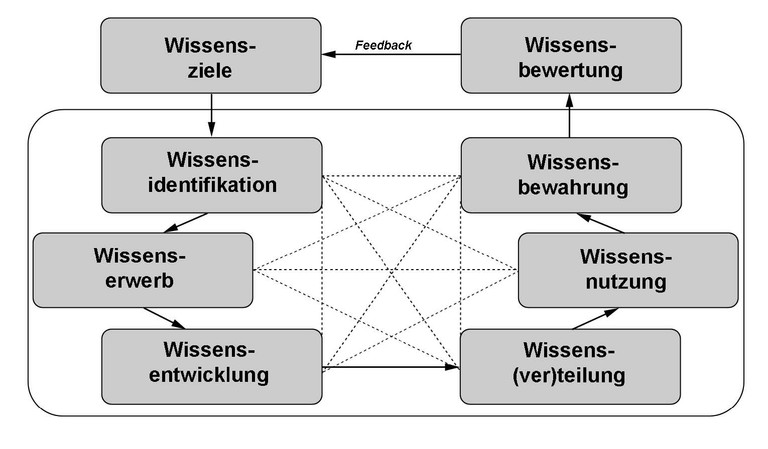
\includegraphics[width=15cm]{kapitel/gruppe2/bilder/wissensmanagament_probst}
	\caption{Bausteinmodell des Wissensmanagement\protect\footnotemark}
	\label{fig_wissensmanagament_probst}
\end{figure}\footnotetext{\cite{wissensmanagement_blog.protechnology.de_2012}}

\subsection{E-Learning}
\label{subsection_e-learning}
E-Learning ist das Lehren und Lernen, welches durch elektronische Medien unterstützt wird. Zum Einsatz kommen digitale Medien, wie zum Beispiel Computer oder Smartphones. Die Übermittlung von Lerninhalten erfolgt über verschiedenste Kanäle wie zum Beispiel das Internet, Computersoftware, Chatsysteme oder durch den Einsatz eines LMS (Learning Management System). Ein sehr bekanntes LMS ist die Plattform Moodle.\footcite[Vgl.][]{e-learning_team025.jimdo.com_2009} In Kapitel \ref{subsubsection_e_learning_plattformen} wird darauf ebenfalls Bezug genommen.

\subsubsection{E-Learning an der Hochschule Emden/Leer}
E-Learning hat an der Hochschule einen hohen Stellenwert, da die Studiengänge Medieninformatik (Online) und seit 2015 Wirtschaftsinformatik (Online) akkreditiert  wurden. Nun soll dargelegt werden, ob in den Präsenzstudiengängen ebenfalls der E-Learning-Prozess Einzug gehalten hat.

\subsubsection{E-Learning in den Präsenzstudiengängen}
Es soll betrachtet werden, in welchen Präsenzstudiengängen E-Learning eingesetzt wird.

Der Fachbereich SAG (Soziale Arbeit und Gesundheit) ist der Vorreiter aller Fachbereiche mit der Einführung eines E-Learning Systems gewesen. SAG setzt mehr als 200 Onlinekurse im Präsenzstudium ein. Für die Anmeldung an verschiedenen Kursen sowie der Klausuranmeldung kommt ein Online-System zum Einsatz.

Es folgt dann der Fachbereich Technik, in dem E-Learning ebenfalls sehr stark verbreitet ist, da die Studiengänge Medieninformatik und Wirtschaftsinformatik als reine Onlinestudiengänge in diesem integriert sind.

Weniger stark wird E-Learning vom Fachbereich Wirtschaft betrieben. Das geringste Nutzungsverhalten ist im Fachbereich Seefahrt zu verzeichnen.

Trotz des unterschiedlichen Nutzungsverhaltens hat E-Learning in allen Fachbereich Einzug gehalten.\footcite{gunter_muller_interview}

\subsubsection[Einsatz von E-Learning-Anwendungen]{Einsatz von E-Learning-Anwendungen in den Präsenzstudiengängen}
In diesem Abschnitt wird erläutert, ob die Anwendungen "'Adobe Connect"' und "'Moodle"' im Präsenzstudiengang eingesetzt werden.\footcite{gunter_muller_interview}

\paragraph{Adobe Connect}\mbox{} \\\\
Adobe Connect ist eine Kommunikationsplattform zur Bereitstellung von Webmeeting- und E-Learning-Inhalten.

Ausschließlich der Fachbereich Technik (E+I) nutzt durch seine Onlinestudiengänge die Plattform Adobe Connect als Medium des visuellen Austausches von Bild und Sprache. In den Präsenzstudiengängen kommt die Plattform nicht zum Einsatz, da der persönliche Austausch von Studierenden und Dozenten in den täglichen Präsenzen stattfindet.\footcite{gunter_muller_interview}
\clearpage

\paragraph{Moodle}\mbox{}\\\\
\label{paragraph_moodle}
Die Hochschule setzt als Lernplattform Moodle ein (siehe Abbildung \ref{fig_moodle}). Moodle ist ein freies objektorientiertes Kursmanagementsystem, welches den Fokus auf E-Learning Inhalte setzt.\footcite{hsel_moodle_2015}

\begin{figure}[h!]
	\centering
	\includegraphics[width=15cm]{kapitel/gruppe2/bilder/moodle}
	\caption{Übersicht Moodle für alle\protect\footnotemark}
	\label{fig_moodle}
\end{figure}\footnotetext{\cite{hsel_moodle_2015}}

Durch den Einsatz von Moodle in allen Fachbereichen wird das volle Leistungsspektrum des Systems ausgenutzt. Folgende Funktionalitäten werden angeboten:

\begin{itemize}
	\item Lernvideos
	\item Vorlesungsskripte
	\item Forum
	\item Kalender
	\item Mail-Connect
\end{itemize}

Für jeden Fachbereich wird der volle Funktionsumfang der Plattform zur Verfügung gestellt, auch wenn nicht jeder Fachbereich jeden Service nutzt.\footcite{gunter_muller_interview} 

\subsubsection{Zentrale Informationsbereitstellung durch Datenlaufwerke}
\label{zentrale_Datenlaufwerke}
Für alle Beteiligten der Hochschule werden drei Datenlaufwerke (siehe Abbildung \ref{fig_zugriff_datenlaufwerke_extern}) auf den Fileservern des eigenen Rechenzentrums zur Verfügung gestellt.\footcite{hsel_moodle_welcome_2015}

\begin{figure}[h!]
	\centering
	\includegraphics[width=15cm]{kapitel/gruppe2/bilder/zugriff_auf_laufwerke_extern}
	\caption{Zugriff auf die Datenlaufwerke von extern \protect\footnotemark}
	\label{fig_zugriff_datenlaufwerke_extern}
\end{figure}\footnotetext{\cite{hsel_moodle_portal_2015}}


\paragraph{Laufwerk Z}\mbox{}\\\\
Auf dem "'Laufwerk Z"' befinden sich die Daten des Home-Verzeichnisses jedes einzelnen Benutzers. Meldet sich dieser an beliebigen Rechnern des internen Rechnerpools an, werden die Inhalte seines Home-Verzeichnisses automatisch eingebunden. Der interne Zugriff auf die eigenen Dateien ist von jedem Rechner des Pools möglich, da servergespeicherte Profile zum Einsatz kommen. Auch von extern können die Studierenden problemlos auf die Ressourcen der Datenlaufwerke zugreifen.\footcite{gunter_muller_interview}

\paragraph{Laufwerk Y}\mbox{}\\\\
Für den gemeinsamen Austausch der Daten wurde das "'Laufwerk Y"' eingerichtet. Hier werden zentral Ressourcen für alle Studierenden und Lehrenden aus Emden zum Austausch zur Verfügung gestellt.\footcite{gunter_muller_interview}
\clearpage
\paragraph{Verzeichnis Lehrende aus Leer}\mbox{}\\\\
Zusätzlich zum Transferlaufwerk wird das Laufwerk "'Verzeichnis Lehrende aus Leer"' zur Verfügung gestellt. Dieses Laufwerk wird zur Bereitstellung von Inhalten (Vorlesungsmaterialien, Skripte, Übungen) verwendet.\footcite{gunter_muller_interview}

\subsubsection{Moodle vs. Datenlaufwerke für Präsenzstudenten}
An der Moodle-Lernplattform melden sich die Nutzer über eine webbasierte Oberfläche am System an. Um Dateien zur Verfügung zu stellen, muss auf der Weboberfläche zu den gewünschten Reitern navigiert werden.

Stellt man die Datenlaufwerke ("'Laufwerk Y"' und das Transferlaufwerk "'Verzeichnis Lehrende aus Leer"') der Moodle-Plattform gegenüber und betrachtet nur den Aspekt des Datenaustausches, so wird deutlich, dass der Dateiaustausch über Datenlaufwerke in Bezug auf Komfort und Aufwand deutlich besser für die Präsenzstudierenden geeignet ist, als die Dateiablage über die Moodle-Plattform. Die über die Datenlaufwerke zur Verfügung gestellten Inhalte können von den Studierenden mit wenig Aufwand intuitiv erreicht werden.

Aus dem Interview mit Günter Müller kristallisierte sich heraus, dass der Fachbereich Wirtschaft die Datenlaufwerke am stärksten sowie der Fachbereich Technik und andere Fachbereiche diese weniger stark nutzen.\footcite{gunter_muller_interview}

\subsection{Sicherheitsaspekte}
\label{subsection_sicherheitsaspekte}
In diesem Kapitel wird auf die bereits verwendeten Sicherheitsrichtlinien an der Hochschule detaillierter eingegangen. Weiterhin wird geprüft, ob ein IT-Service-Management-Prozess  umgesetzt ist.

\subsubsection{Sicherheitsrichtlinien an der Hochschule}
Der Einsatz von Sicherheitsrichtlinien ist ein wichtiges Thema an Hochschulen. Sicherheitsrichtlinien beschreiben die Sicherstellung von Verfügbarkeit, Integrität, Vertraulichkeit und Authentizität von Informationen.\footcite[Vgl.][]{sicherheitsrichtlinien_datenschutz-berlin.de_2008}

An der Hochschule werden, als Basis für die Informationssicherheit, Teile des IT-Grund-schutz-Kataloges umgesetzt. Nicht alle Empfehlungen des BSI (Bundesamt für Sicherheit in der Informationstechnik) sind an einer kleinen Hochschule, wie die Hochschule Emden/Leer es ist,  umsetzbar. Das BSI ist eine nationale Sicherheitsbehörde deren Ziel es ist, die IT-Sicherheit in Deutschland voran zu bringen. Somit ist das BSI ein zentraler IT-Sicherheitsdienstleister des Bundes.\footcite[Vgl.][]{sicherheitsrichtlinien_bsi.bund.de_2015}

An den Serverräumen der Hochschule ist die Umsetzung der IT-Grundschutzmaßnahmen deutlich zu erkennen.
Folgende physikalische Schutzmaßnahmen wurden in den Serverräumen umgesetzt\footcite{gunter_muller_interview}:

\begin{itemize}
	\item einbruchssicher
	\item feuergemeldet
	\item videoüberwacht
	\item Lage der Serverräume im ersten Obergeschoss (Wasserschutz)
\end{itemize}

\subsubsection{Einsatz von ITIL}
Die IT Infrastructure Libary (ITIL) ist eine Sammlung von Best Practises zur Umsetzung eines IT-Service-Management-Prozesses (siehe Kapitel \ref{subsubsection_ITIL}). In diesem Regelwerk werden die für den Betrieb einer IT-Infrastruktur notwendigen Prozesse und Werkzeuge beschrieben.\footcite[Vgl.][]{itil_dxperts.de_2015} ITIL gilt als De-Facto-Standard. Eine Zertifizierung ist nicht für Unternehmen, sondern nur für Personen möglich. Unternehmen können sich nach ISO 20000 zertifizieren lassen.\footcite[Vgl.][]{itil_wirtschaftslexikon.gabler}

Der ITIL-Prozess ist an der Hochschule nicht umgesetzt, da die Personaldecke für die Umsetzung eines 1st- und 2nd-Level Supports nicht gegeben ist.\footcite{gunter_muller_interview}

\subsubsection{Umsetzung von ISO/IEC 27001}
Die ISO/IEC 27001 Zertifizierung wird auf Basis des IT-Grundschutzes vergeben. Durch die Zertifizierung des ISO/IEC 27001 Standards haben Unternehmen, Behörden und Organisationen die Möglichkeit, ihre Bemühungen um Informationssicherheit nach innen und außen zu dokumentieren.\footcite[Vgl.][]{iso_27001_bsi.bund.de_2015}

Das Einsatzszenario ist an der Hochschule nicht gegeben, da für Umsetzung die Personaldichte zu gering ist. Für die Erfüllung der Zertifizierung würde ein riesiger Personaloverhead entstehen.\footcite{gunter_muller_interview}

\subsubsection{Fazit Sicherheitsrichtlinien}
Abschließend ist zu sagen, dass an der Hochschule der IT-Sicherheitsaspekt eine sehr entscheidende Rolle spielt. Als kleine Hochschule ist es auf Grund der Personaldichte nicht möglich, alle Empfehlungen des BSI-Grundschutzes, ITIL und ISO/IEC 27001 umzusetzen. Jedoch sucht sich die Hochschule aus den Regelwerken die Empfehlungen heraus, die auf Grund der Personaldichte umsetzbar sind. Dies bildet eine sehr gute Basis im Hinblick auf das sehr anspruchsvolle Thema IT-Sicherheit.
\section{Repräsentation von Informationen (TK)}
Ein wichtiger Aspekt an Hochschulen ist die Repräsentation von Informationen. Hier spielt sowohl das 
Erscheinungsbild nach außen, als auch die Repräsentation von Informationen innerhalb der einzelnen Bereiche 
eine entscheidende Rolle. Für die interne und externe Kommunikation ist der Bereich "'Presse- und 
Öffentlichkeitsarbeit"' der Hochschule zuständig (siehe Kapitel \ref{praesidium_label}). Nachfolgend wird auf 
die Teilbereiche Studentengewinnung, Corporate Identiy und das Handling von Bewerberdaten näher 
eingegangen.

\subsection{Studentengewinnung}
Wie in Kapitel \ref{praesidium_label} bereits erwähnt, obliegt die Zuständigkeit des Marketings dem 
Präsidialbüro. Generell ist die Studentengewinnung wie folgt aufgeteilt: Zum einen existiert eine zentrale 
Studienberatung, bei der sich Interessenten direkt informieren können und zum anderen werden regelmäßig 
Besuche von Mitarbeitern der Hochschule an Schulen der Region durchgeführt. Mitglieder der Fachbereiche 
berichten vor Ort in den Schulen über die Inhalte der jeweiligen Studiengänge. Neben diesen beiden 
Maßnahmen zur Studentengewinnung verfügt die Hochschule ebenso über Onlinemedien, mit deren Hilfe sich 
die Interessenten über den gewünschten Studiengang und den generellen Ablauf des  Studiums informieren 
können.\footcite[Vgl.][]{gunter_muller_interview}


\subsection{Corporate Identity}
Die Hochschule hat eine Corporate Design-Regelung, die auf der Webseite öffentlich eingesehen werden 
kann. Diese wird vom Bereich Marketing zur Verfügung gestellt und 
gepflegt.\footcite[Vgl.][]{hsel_CD}
\clearpage

Die CD-Reglung umfasst unter anderem einen 
CD-Regelungsguide\footcite{hsel_CD_manual} sowie diverse Vorlagen für PowerPoint 
Präsentationen bis hin zu allgemeinen Logos sowie angepasste Logos für jeden Fachbereich (siehe Abbildung 
\ref{fig_logo_allgemein} und \ref{fig_logo_fb_technik}).

\begin{figure}[h!]
	\centering
	\includegraphics[width=8cm]{kapitel/gruppe2/bilder/hs_logo_allgemein}
	\caption{Allgemeines Logo der Hochschule Emden/Leer\protect\footnotemark}
	\label{fig_logo_allgemein}
\end{figure}\footnotetext{\cite{hsel_CD_manual}}

\begin{figure}[h!]
	\centering
	\includegraphics[width=8cm]{kapitel/gruppe2/bilder/hs_logo_technik}
	\caption{Logo des Fachbereiches Technik\protect\footnotemark}
	\label{fig_logo_fb_technik}
\end{figure}\footnotetext{\cite{hsel_CD_manual}}

\subsection{Handling von Bewerberdaten}
Durch das Interview mit Günter Müller wurde festgestellt, wie das allgemeine Handling von Bewerberdaten aus Sicht des Rechenzentrums stattfindet. 
Der Bewerber meldet sich mit seinen bei Registrierung erstellten Daten am Hochschulinformationssystem (HIS) der Hochschule an und der generierte Account ist nur für die Dauer des Bewerbungszeitraumes aktiv. Im Fall der Nichtannahme des Bewerbers, erfolgt im Anschluss die Löschung seines Accounts. Bei Immatrikulation des Bewerbers wird der vorhandene temporäre Account in einen permanenten Account mit erweiterten Informationseingaben umgewandelt (z.B. Krankenkassendaten). Auf diese Weise wird sichergestellt, dass nur aktive Studenten einen Account zur Verfügung gestellt bekommen.\footcite[Vgl.][]{gunter_muller_interview}
\clearpage
\section{Kooperations-Situation mit anderen Hochschulen (ME)}
\label{section_kooperations_situation}

Das Kooperationsverhältnis mit anderen Hochschulen, Verbänden und Unternehmen spielt auch an der Hochschule Emden/Leer eine sehr entscheidende Rolle, da durch die Kooperation verschiedene Services zur Verfügung gestellt werden.

\subsection{Regionaler Bezug zu Hochschulen (Mitgliedschaften)}
Die Hochschule pflegt ein enges Kooperationsverhältnis mit dem Jade-Hochschulverbund. Über das LBS (Lokale Bibliothekssystem Ostfriesland/Wilhelmshaven) wird auf die gemeinsamen  Bibliotheksbestände zugegriffen.\footcite{jadehs_online_kataloge_2015} Durch ein gemeinsames Promotionskolleg findet ebenfalls eine intensive Zusammenarbeit mit der Universität Vechta statt. Aktuell wird die Kooperation zur Hochschule Osnabrück ausgebaut.\footcite[Vgl.][]{hsel_profil_2015}

Der Rechenzentrumsleiter Herr Günter Müller ist selbst Mitglied des Arbeitskreises LANIT/HRZ.\footcite[Vgl.][]{lanit_mitglieder_2011} Hier treffen die Leiter der Rechenzentren Niedersachsens aufeinander und tauschen ihre Erfahrungen aus. Der Arbeitskreis befasst sich mit Themen der IT-Infrastruktur für Forschung, Lehre und Verwaltung an den Hochschulen Niedersachsens. Zu verschieden Schwerpunktthemen wurden in dem Arbeitskreis entsprechende Arbeitsgruppen eingerichtet.  Ebenfalls werden hochschulübergreifend Projekte durchgeführt.\footcite[Vgl.][]{lanit_home_2014}

Das ZKI (Zentren für Kommunikation und Informationsverarbeitung in Lehre und Forschung e.V.) spielt für die Hochschule eine wichtige Rolle. Ziel dieses Vereins ist es, die Kooperation zwischen den ZKI/Rechenzentren, Meinungs- und Erfahrungsaustausch, sowie die Beratung und Zusammenarbeit mit bildungs- und wirtschaftsfördernden Einrichtungen zu fördern. In den immer wiederkehrenden Tagungen erarbeitet der Arbeitskreis Lösungsvorschläge für aktuelle Probleme der Informationsverarbeitung.\footcite[Vgl.][]{zki_verein_2015} Aktuelle Themen sind z.B. eine Studie über das Thema: „CIOs und IT-Governance an deutschen Hochschulen“.\footcite{zki_beitrag_CIOs_2014}

Durch den Verein DFN (Deutsches Forschungsnetz) wird der Hochschule eine Vielzahl von maßgeschneiderten Kommunikationsanwendungen (DFN-Diensten) zur Verfügung gestellt. Der DFN-Verein ist ein von der Wissenschaft selbst organisiertes Kommunikationsnetz für Wissenschaft und Forschung in Deutschland. Er verbindet Hochschulen und Forschungseinrichtungen miteinander und ist in den europäischen und weltweiten  Verbund der Forschungsnetze integriert.\footcite[Vgl.][]{dfn_home_2015}

\subsection{Kooperation zwischen Unternehmen}
Regional betrachtet, arbeitet die Hochschule mit 82\% der Unternehmen der Region zusammen. Der Vorteil dieser Kooperation ist es, dass zum einen die Studierenden die Möglichkeit haben ihre Fähigkeiten in der Praxis anzuwenden und zum anderen können die Unternehmen das Know-How  der Hochschule nutzen und sinnvoll einsetzen. Der Wissenstransfer, der in der Hochschule erfolgt, bietet den Unternehmen einen erheblichen Mehrwert.\footcite[Vgl.][]{hsel_artikel_kooperation_unternehmen_2014}

\subsection{Eingesetzte IT-Systeme durch Mitgliedschaft im DFN-Verein}
Die angebotenen Dienste des Deutschen Forschungsnetzes sind für den Zweck von Wissenschaft und Forschung maßgeschneidert worden. Ein besonderes Augenmerk liegt hier auf der guten Integration der Dienste in die Prozesse der Hochschulen.  Auf die über den DFN-Verein zur Verfügung gestellten Dienste, die an der Hochschule Emden/Leer zum Einsatz kommen, wird folgend näher eingegangen.\footcite[Vgl.][]{dfn_dienste_2014}

\subsubsection{DFNRoaming/eduroam}
Die Hochschule ist Mitglied des Deutschen Forschungsnetzes (DFN).\footcite{dfn_mitgleider_2012} Durch diese Kooperation nutzt die Hochschule den durch das DFN zur Verfügung gestellten Dienst DFNRoaming/eduroam. Dieser ermöglicht es, registrierten Nutzern über dienst-konforme WLANs Zugang zum Wissenschaftsnetz zur Verfügung zu stellen. Der DFN-Verein betreibt und pflegt die eduroam Förderationsserver in Deutschland. \footcite[Vgl.][]{dfn_roaming_2015} 

In der Abbildung \ref{fig_map_eduroam} ist ein Ausschnitt der weltweiten Lokalitäten der Förderationsserver dargestellt.

\begin{figure}[h!]
	\centering
	\includegraphics[width=\textwidth]{kapitel/gruppe2/bilder/eduroam_map}
	\caption{Standorte der Länder, in denen DFNRoaming/eduroam betrieben wird\protect\footnotemark}
	\label{fig_map_eduroam}
\end{figure}\footnotetext{\cite{weill_cornell_eduroam_2015}}

\subsubsection{GigaMove der RWTH Aachen}
\label{gigamove_rwth_aachen}
Die RWTH Aachen (Rheinisch-Westfälische Technische Hochschule Aachen) stellt eine einfach zu nutzende Möglichkeit zum kurzfristigen Austausch großer Dateien zur Verfügung. Der Datenaustausch kann aus zwei Richtungen erfolgen. Zum einen kann die Nutzer eine Datei hochladen und das System erzeugt einen Link zum Download, zum anderen kann eine Datei angefordert werden, bei der das System einen Link generiert, der zu einem Formular zum Upload der Datei führt. Jeder Nutzer darf Dateien in der Gesamtgröße von 10 GB für einen Zeitraum von 14 Tagen auf den Servern abspeichern. Der von der RWTH Aachen gehostete Dienst GigaMove wird den Nutzern der Hochschule zur Verfügung gestellt.\footcite{hsel_servicelinks_2015} In der Abbildung \ref{fig_rwth_gigamove} ist die Plattform GigaMove der RWTH Aachen dargestellt.

\begin{figure}[h]
	\centering
	\includegraphics[width=\textwidth]{kapitel/gruppe2/bilder/rwth_gigamove}
	\caption{Übersicht der Plattform GigaMove der RWTH Aachen \protect\footnotemark}
	\label{fig_rwth_gigamove}
\end{figure}\footnotetext{\cite{rwth_aachen_gigmove_2015}}

\subsubsection{DFNVideoConference (DFNVC)}
DFNVC (Deutsches Forschungsnetz Video Conference) bietet den Nutzern die Möglichkeit von einem 
PC, einem Raumsystem oder einem Telefon vom Hochschulstandort, durch die Nutzung des 
Wissenschaftsnetzes X-WiN, mit einem oder mehreren Nutzern zu kommunizieren. Die Kommunikation 
findet multimedial statt. Das Wissenschaftsnetz X-WiN ist die technische Plattform des Deutschen 
Forschungsnetzes. Über das X-WiN sind die Hochschulen und Forschungseinrichtungen in Deutschland 
untereinander und mit den Wissenschaftsnetzen in Europa und auf anderen Kontinenten 
vernetzt.\footcite[Vgl.][]{dfn_DFNVideoConference_2014} An der Hochschule wird dieser Dienst 
ebenfalls genutzt\footcite{hsel_shibboleth_auth_2015} und ist über einen Link auf die 
Hochschulwebsite erreichbar.\footcite{dfn_DFNVC_Webkonferenzen_2015}

\subsection{Authentifizierung über Shibboleth-Verfahren und Single-Sign-On}
\label{shibboleth_sso} 

Das Shibboleth-Verfahren (Verfahren zur Verteilten Authentifizierung und Autorisierung für 
Webanwendungen) kommt an der Hochschule zum Einsatz.\footcite[Vgl.][]{hsel_shibboleth_auth_2015}  
Durch dieses Verfahren können Dienste bestimmter Anbieter mit dem Hochschullogin genutzt werden, 
ohne dass bei diesem Anbieter ein neuer Account (Benutzerkennung und Passwort) erstellt werden 
muss. Hierfür existiert an der Hochschule ein Identity Provider Dienst und bei dem entsprechenden 
Dienstanbieter ein Service Provider Dienst.  Beim Aufruf einer Dienstanbieter-Ressource prüft der 
Service Provider Dienst, ob eine bestehende Anmeldesession existiert und leitet die Anfrage an die zur 
Verfügung gestellten Ressourcen weiter, ist dies nicht der Fall, wird der Benutzer an auf Seite 
weitergeleitet, wo er die Lokalität seiner Hochschule auswählen muss. Nach erfolgter Auswahl wird die 
Anfrage an den Identity Provider Dienst der ausgewählten Lokation 
weitergeleitet.\footcite[Vgl.][]{kit_shibboleth_2012} Wie in Abbildung \ref{fig_shibboleth_hs} 
dargestellt, ist dann für eine erfolgreiche Anmeldung die Hochschulkennung erforderlich. Es wird also 
ein zentralisierter Account für die Authentifizierung genutzt.  

\begin{figure}[h]
	\centering
	\fbox{\includegraphics[width=10cm]{kapitel/gruppe2/bilder/shibboleth}}
	\caption{Shibboleth-Login der Hochschule \protect\footnotemark}
	\label{fig_shibboleth_hs}
\end{figure}\footnotetext{\cite{hsel_shibboleth_auth_2015}}
\clearpage
Das Shibboleth-Verfahren ermöglicht den Studierenden und Mitarbeitern die Nutzung folgender Dienste \footcite{hsel_shibboleth_vpn_2015} :

\begin{itemize}
	\item DFNVC (DFN-Webkonferenzen)
	\item Gigamove
	\item video2brain
	\item Springer Link	
	\item WISO	
\end{itemize}

Single-Sign-On, wie in Kapitel \ref{realisierung_der_serviceorientierung} beschrieben, findet in Verbindung mit dem Shibboleth-Verfahren Verwendung. Nach erfolgreicher Authentifizierung ist der Zugriff auf alle Dienstanbieter-Ressourcen, die der Hochschule zur Verfügung stehen, möglich. Es müssen keine weitere Anmeldedaten eingegeben werden.

Für den Zugriff auf die Datenlaufwerke (siehe Kapitel \ref{zentrale_Datenlaufwerke}) wird ebenfalls Single-Sign-On verwendet, da nach der Anmeldung am Client keine weiteren Benutzerdaten zur Authentifizierung eingegeben werden müssen. 
\newpage
\subsubsection{Springer Link}
Studierende und Mitarbeiter der Hochschule haben über die Springer Link-Kooperation Zugriff auf über 40.000 Bücher, 5 Millionen Artikel, 2200 Zeitschriften und 165 Nachschlagewerk.\footcite{springer_springerlink_faq_2015} Die Oberfläche der Springer Link Plattform ist in Abbildung \ref{fig_springerlink_startseite} zu sehen. Springer Link bietet die Möglichkeit die Inhalte als *.pdf herunterzuladen. 

\begin{figure}[h]
	\centering
	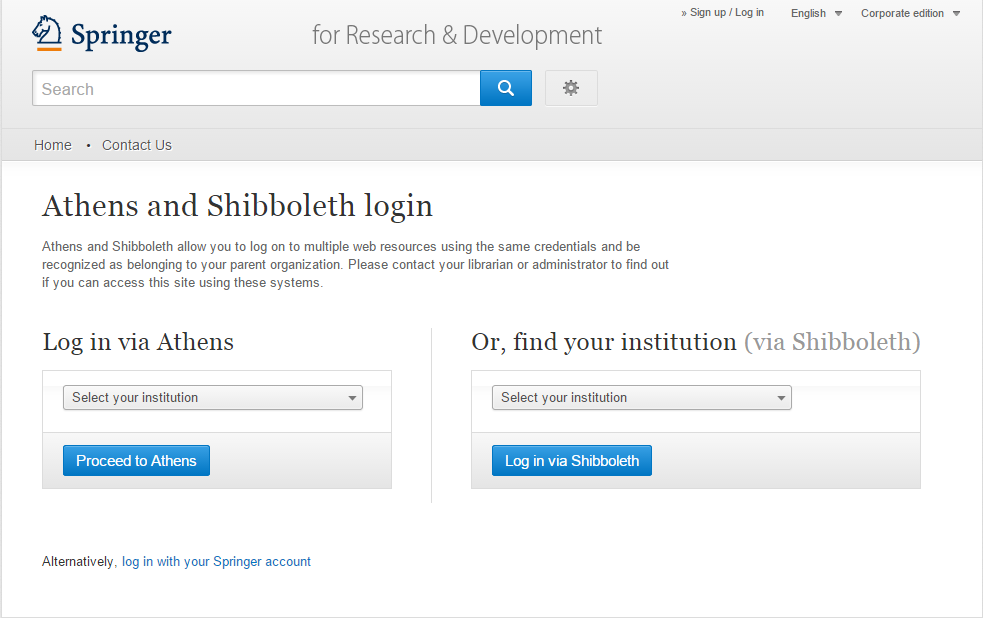
\includegraphics[width=\textwidth]{kapitel/gruppe2/bilder/springerlink_startseite}
	\caption{Springer Link Startseite \protect\footnotemark}
	\label{fig_springerlink_startseite}
\end{figure}\footnotetext{\cite{springer_login_athens_2015}}
\clearpage
\subsubsection{WISO}
Durch das Kooperationsverhältnis mit der GBI-Genios Deutsche Wirtschaftsdatenbank GmbH können die Mitglieder der Hochschule das komplette Angebot an Fachinformationen zu Wirtschafts- und Sozialwissenschaften, technischen Studiengängen und zur Psychologie  nutzen. WISO bietet über 14 Mio. Literaturnachweise, 2100 elektronische Bücher, 130 Mio. Artikel, 700.000 Marktdaten.\footcite{gbi_genios_uber_wiso_2015} Die WISO-Plattform ist in Abbildung \ref{fig_wiso_plattform} zu sehen.

\begin{figure}[h]
	\centering
	\includegraphics[width=\textwidth]{kapitel/gruppe2/bilder/wiso_plattform}
	\caption{Übersicht der WISO-Plattform \protect\footnotemark}
	\label{fig_wiso_plattform}
\end{figure}\footnotetext{\cite{gbi_genios_homepage_2015}}
\newpage
\subsubsection{video2brain}
Seit 2015 ist für alle Mitarbeiter und Studierende der Zugang zum Videostreaming-Portal der video2brain GmbH möglich. Schwerpunkt sind IT- und Kreativ-Themen, Lehrvideos für Fotografen, Grafiker, Web- und Screendesigner. Das Verlagsangebot umfasst mehr als 1700 Video-Trainingskurse. \footcite{adsgmbh_video2brain_2013} In der Abbildung \ref{fig_video2brain_suchergebnis} ist die Weboberfläche nach erfolgreicher Shibboleth-Authentifizierung dargestellt.

\begin{figure}[h]
	\centering
	\includegraphics[width=\textwidth]{kapitel/gruppe2/bilder/video2brain_suche}
	\caption{Übersicht der video2brain Plattform \protect\footnotemark}
	\label{fig_video2brain_suchergebnis}
\end{figure}\footnotetext{\cite{video2brain_homepage_2015}}

\subsection{Support der Dienste}
Für die zentral angebotenen Dienste eduroam, Shibboleth und GigaMove übernimmt die Hochschule den Endkundensupport. Die Mitarbeiter der Hochschule bilden somit die zentrale Support-Schnittstelle und delegieren Anfragen, die vor Ort nicht gelöst werden können, an die entsprechenden Anbieter und Dienstleister weiter.

Diese teilte uns Günter Müller in dem durchgeführten Interview mit.
\section{Bewertung und Gewichtung (TK)}
Abschließend kann gesagt werden, dass Informationen zentral gesammelt werden und wichtige Systeme wie das "'Laufwerk Y"' und die E-Learning Plattform (Moodle) in allen Fachbereichen und in Teilen der Verwaltung zum Einsatz kommen. Durch den starken Kooperationsverbund werden zentrale Dienste, wie Springer Link, WISO und video2brain für die Studierenden und Mitarbeiter dezentral zur Verfügung gestellt. 

Bei der Repräsentation von Informationen nach außen verfügt die Hochschule über eine Pressestelle und eine Marketingabteilung. Es existiert eine feste CD-Reglung für alle Abteilungen und Bereiche. 

Durch diverse Arbeitsgruppen ist der Erfahrungs-, Wissens- und Informationsaustausch für wichtige Bereiche bereits gegeben. Durch die Arbeitsgruppe ZDF, WEB und Moodle werden zentrale Systeme zur Wissenserhaltung und Informationsbereitstellung gepflegt. Dadurch, das die Arbeitsgruppen abteilungsübergreifend agieren, besteht auch zwischen den einzelnen Bereichen eine Schnittstelle, ohne die autarken Fachbereiche einzuschränken. 

Im Bezug auf Serviceorientierung und IT-Sicherheit lässt sich sagen, dass SSO (Single-Sign-On) für einige Bereiche bereits zum Einsatz kommt (siehe Kapitel \ref{realisierung_der_serviceorientierung}). Ebenso werden Teile des IT-Grundschutzes erfolgreich an der Hochschule eingesetzt. Dies sind erste Schritte zum Informationsmanagement, jedoch fehlt grundsätzlich ein zentrales System für den direkten Zugriff und zur Weiterleitung auf weitere Informationssysteme. In Kapitel \ref{immatrikulations_und_pruefungsamt} wird beschrieben, dass in Hochschulen, welche ein Informationsmanagement einsetzen, dieses meistens im Bereich Immatrikulations- und Prüfungsamt (HIS) angesiedelt ist. 
Neben einem  zentralem System fehlt auf der organisatorischen Seite eine Instanz. Wie in Kapitel \ref{cio_text} beschrieben, findet im klassischen Informationsmanagement für Unternehmen das Management häufig durch einen CIO (Chief Information Officer) statt. In Hochschulen wird dies oft durch DACH Organisationen realisiert. 

Auch wenn die Hochschule bereits diverse Arbeitsgruppen einsetzt, so ist diese Instanz des Informationsmanagements bisher unbesetzt. Ein Informationsmanagement, wie es in Kapitel \ref{begriffsdefintion_inm} beschrieben ist, wird derzeit an der Hochschule nicht vollständig praktiziert.